%%% preamble
\documentclass[12pt]{article}

%% packages
\usepackage{graphicx}

%% title
\title{Static \textbf{leaflet} map using \textbf{knitr}}
\author{\vspace{-10ex}}
\date{\vspace{-5ex}}


%%% document
\usepackage{Sweave}
\begin{document}
\Sconcordance{concordance:png_in_latex.tex:png_in_latex.Rnw:%
1 11 1 49 0 1 3 12 1 4 0 1 1 1 20 7 1}


%% global chunk options

\maketitle

This is an example on how to display static \textbf{leaflet} maps using \LaTeX.

%% unevaluated leaflet code, create map
\begin{Schunk}
\begin{Sinput}
> m <- leaflet() %>%
+   addTiles() %>%
+   addMarkers(lng = -77.03673, lat = 38.89761)
> m
\end{Sinput}
\end{Schunk}

%% evaluated leaflet code, create map and save as png

%% display image
\begin{figure}[!htbd]
  \begin{center}
    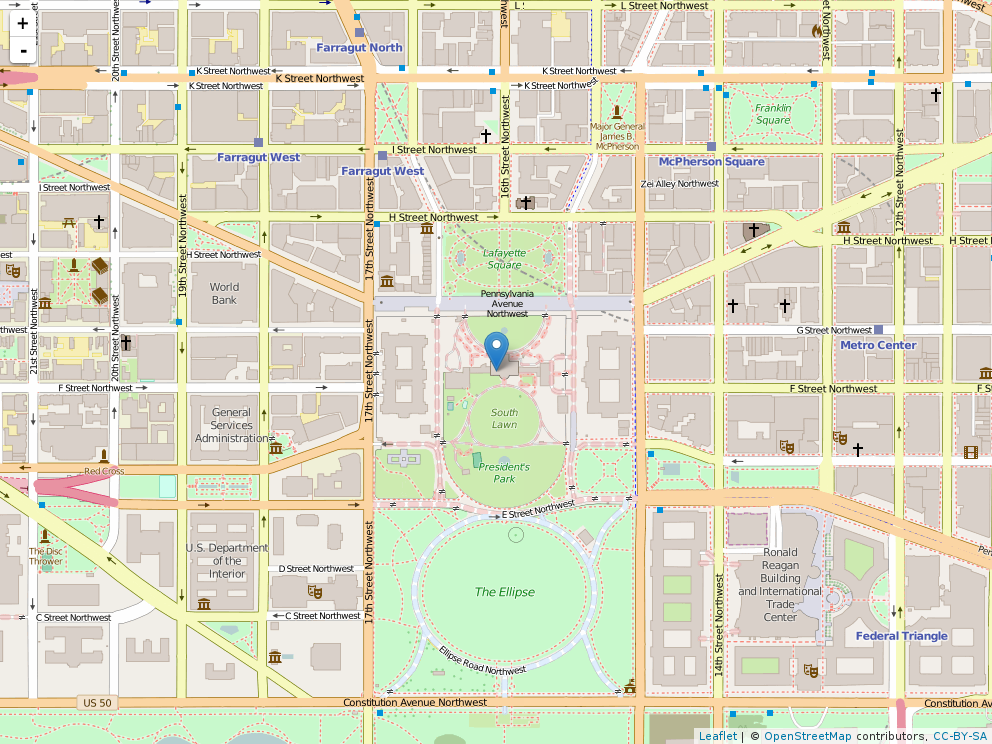
\includegraphics[width = 0.75\textwidth]{leaflet_map.png}
    \caption{Static \textbf{leaflet} map.}
  \end{center}
  \end{figure}
  
\end{document}
